\newpage
\section{Order}
Orders are a new feature in Salespoint 2011. The intention was to prepare the old databaskets for development of web applications and extend them to collaborate with our new inventory, providing the opportunity of individual pricing, final payment and basic log functionality.

Therefore we created the \code{OrderEntry} as main data structure to access these functionality. An \code{OrderEntry} represents one order and can be imagined as sheet of paper which basically consists of lines representing the ordered products (\code{OrderLine}) and lines that are not bound to a concrete product but which cause charge (\code{ChargeLine}). \code{ChargeLines} make it possible to add individual charge to orders. For example they can be used to define forwarding charges or other special charges produced by this order. 

\vskip 1cm
\begin{figure}[ht]
	\centering
  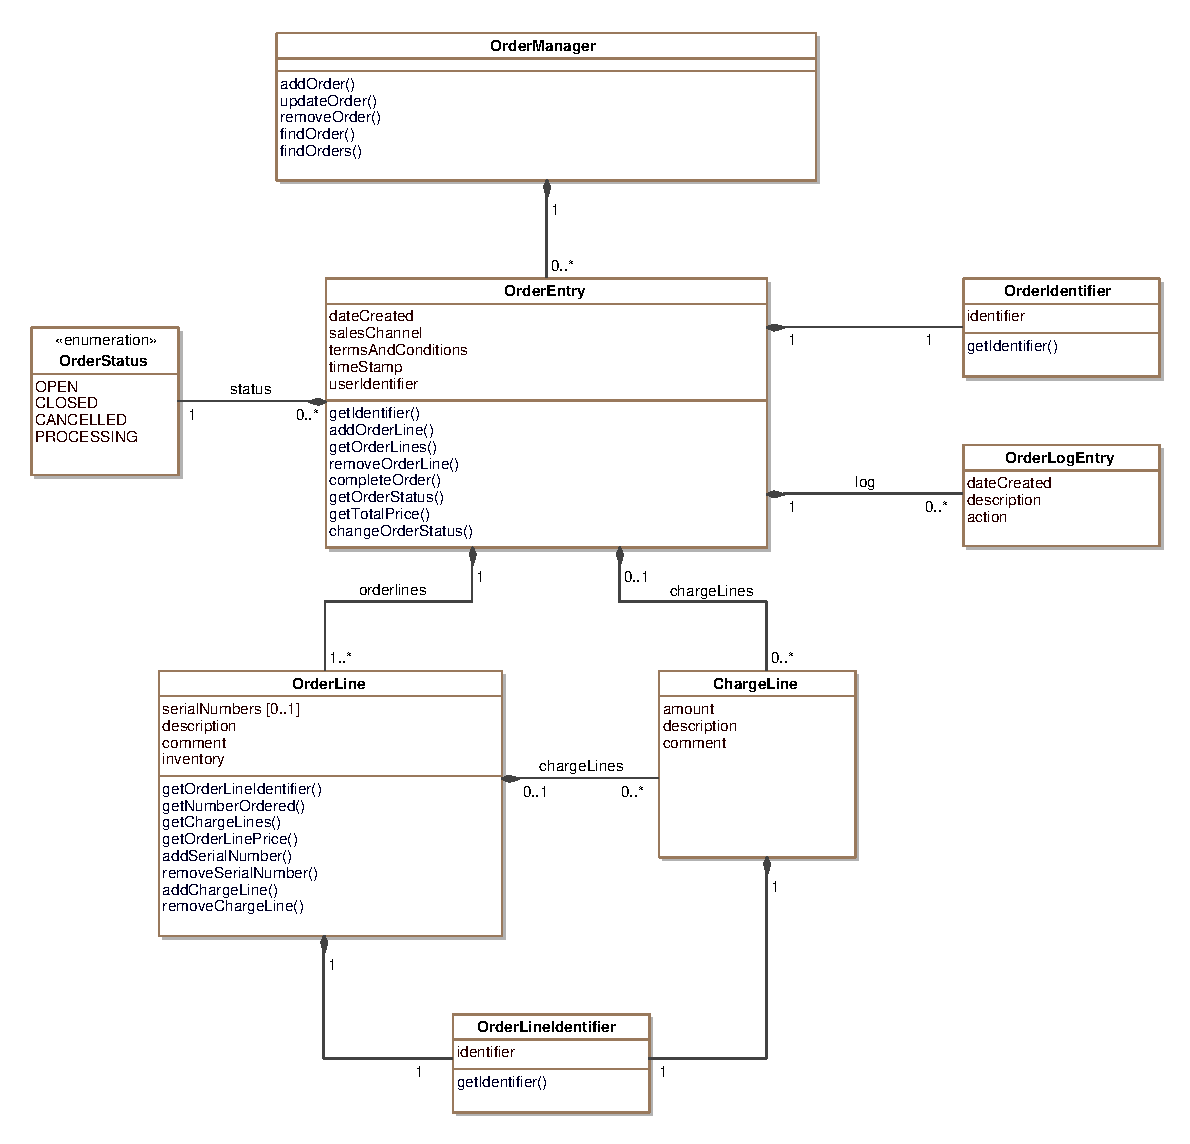
\includegraphics[scale =.7]{images/Overview_Order.eps}
	\label{order_overview}
	\caption{Order - Class Overview}
\end{figure}

\code{OrderEntrys} are lifecycle-objects. The lifecycle covers four states which are defined by enumeration type \code{OrderEntryStatus}. After all the lifecycle has no restrictions in changing states with one exception: \code{CLOSED} is a final state and it's not possible to change the state of \code{CLOSED} \code{OrderEntrys}. The state machine below shows an example of a frequently practised lifecycle.

\vskip 1cm
\begin{figure}[ht]
	\centering
  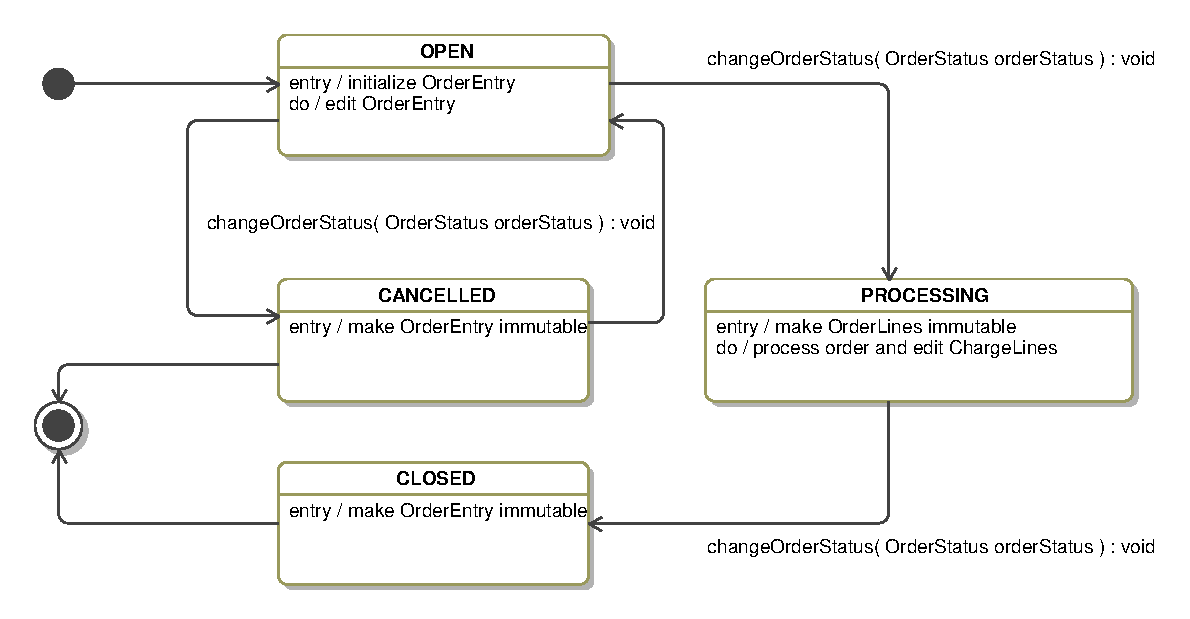
\includegraphics[scale =.7]{images/OrderEntryState.eps}
	\label{order_statemachine}
	\caption{Order - Lifecycle}
\end{figure}  

As you can see an OrderEntry can only completely modified in state \code{OPEN}. \code{CANCELLED} and \code{CLOSED} \code{OrderEntrys} are immutable! An \code{PROCESSING} \code{OrderEntry} is basically also immutable but their is still the possibility to modify the \code{ChargeLines} of that \code{OrderEntry}. 
